\documentclass[11pt,a4paper]{article}

% ── Packages ──────────────────────────────────────────────────────────
\usepackage[utf8]{inputenc}
\usepackage[T1]{fontenc}
\usepackage{lmodern}
\usepackage[margin=2.4cm]{geometry}
\usepackage{amsmath,amssymb,mathtools}
\usepackage{booktabs}
\usepackage{enumitem}
\usepackage{graphicx}
\usepackage{xcolor}
\usepackage{hyperref}
\usepackage{fancyhdr}
\usepackage{listings}
\usepackage{float}
\usepackage{caption}
\usepackage{tcolorbox}
\usepackage{tikz}
\usetikzlibrary{shapes.geometric, arrows.meta, positioning, calc, fit, backgrounds}

% ── Colours ───────────────────────────────────────────────────────────
\definecolor{cBlue}{HTML}{2D6A8A}
\definecolor{cGreen}{HTML}{2D6B4A}
\definecolor{cOrange}{HTML}{C07030}
\definecolor{cPurple}{HTML}{724D8A}
\definecolor{cRed}{HTML}{BF4A4A}
\definecolor{cNavy}{HTML}{1D4A72}
\definecolor{cDarkGreen}{HTML}{145548}
\definecolor{cGray}{HTML}{4A4A4A}
\definecolor{codeGray}{HTML}{F5F5F5}

% ── Hyperref ──────────────────────────────────────────────────────────
\hypersetup{
  colorlinks=true,
  linkcolor=cBlue,
  citecolor=cGreen,
  urlcolor=cNavy,
  pdftitle={PCI Calculator -- Supplementary Material},
  pdfauthor={Berke Isler},
}

% ── Code listings ─────────────────────────────────────────────────────
\lstset{
  basicstyle=\small\ttfamily,
  backgroundcolor=\color{codeGray},
  frame=single,
  rulecolor=\color{gray!30},
  breaklines=true,
  numbers=left,
  numberstyle=\tiny\color{gray},
  keywordstyle=\color{cBlue}\bfseries,
  commentstyle=\color{cGreen}\itshape,
  stringstyle=\color{cOrange},
  language=Python,
  showstringspaces=false,
  tabsize=4,
}

% ── Headers ───────────────────────────────────────────────────────────
\pagestyle{fancy}
\fancyhf{}
\fancyhead[L]{\small\textcolor{gray}{PCI Calculator --- Supplementary Material}}
\fancyhead[R]{\small\textcolor{gray}{February 2026}}
\fancyfoot[C]{\small\thepage}
\renewcommand{\headrulewidth}{0.4pt}

% ── tcolorbox styles ─────────────────────────────────────────────────
\tcbset{
  boxrule=0.5pt,
  arc=3pt,
  left=6pt,
  right=6pt,
  top=6pt,
  bottom=6pt,
  fonttitle=\bfseries,
}

% ══════════════════════════════════════════════════════════════════════
\begin{document}

% ── Title ─────────────────────────────────────────────────────────────
\begin{center}
  {\LARGE\bfseries Perturbational Complexity Index (PCI) Calculator}\\[6pt]
  {\Large Supplementary Material}\\[12pt]
  {\large Berke Isler}\\[4pt]
  {\small\texttt{mehmetberkeisler@gmail.com}}\\[6pt]
  {\small February 2026}\\[4pt]
  \rule{0.6\textwidth}{0.4pt}
\end{center}

\vspace{6pt}

% ── Abstract ──────────────────────────────────────────────────────────
\begin{abstract}
\noindent
This document provides supplementary material for the Perturbational Complexity Index (PCI) Calculator software.
It describes the theoretical background behind PCI, the complete mathematical formulation of the algorithm as
proposed by Casali et al.\ (2013), the implementation details of our Python-based processing pipeline, the
corrections and improvements applied during code review, and a formal description of the \emph{istisna}
exception-handling mode for mislabelled trigger markers. A TikZ-rendered flowchart of the full algorithm
is provided along with pseudocode for all core routines.
\end{abstract}

\tableofcontents
\newpage

% ══════════════════════════════════════════════════════════════════════
\section{Introduction}
\label{sec:intro}

The Perturbational Complexity Index (PCI) is an electrophysiological measure of brain complexity
proposed by Casali et al.\ \cite{casali2013} as a theory-grounded indicator of the level of
consciousness. It builds on the Integrated Information Theory (IIT) prediction that consciousness
requires both \emph{integration} (widespread causal interactions) and \emph{differentiation}
(a large repertoire of distinct states) within the thalamocortical system.

PCI operationalises this by combining two ingredients:

\begin{enumerate}[leftmargin=2em]
  \item \textbf{Perturbation} --- A transcranial magnetic stimulation (TMS) pulse directly
        activates a cortical region, triggering a cascade of evoked activity recorded by
        high-density EEG.
  \item \textbf{Complexity measurement} --- The spatiotemporal pattern of significant cortical
        responses is binarised, then compressed using the Lempel--Ziv algorithm (LZ76). The
        normalised compression ratio yields a single number, PCI $\in [0, 1]$.
\end{enumerate}

Casali et al.\ demonstrated that PCI reliably discriminates conscious from unconscious brain
states across diverse conditions: wakefulness, REM and NREM sleep, anaesthesia (midazolam,
propofol, xenon), locked-in syndrome, vegetative state (VS/UWS), and minimally conscious
state (MCS). A threshold of PCI$^* = 0.31$ was never exceeded during confirmed unconsciousness.

This software implements the full PCI pipeline in Python using MNE-Python for EEG processing,
NumPy for numerical computation, and Streamlit for the interactive web interface.

% ══════════════════════════════════════════════════════════════════════
\section{Mathematical Formulation}
\label{sec:math}

\subsection{Source Entropy}

Given a binary significance matrix $\mathbf{SS}(x, t) \in \{0, 1\}^{L_1 \times L_2}$ where
$L_1$ is the number of sources and $L_2$ the number of post-stimulus time samples, define:

\begin{equation}
  p_1 = \frac{1}{L} \sum_{x=1}^{L_1} \sum_{t=1}^{L_2} \mathbf{SS}(x, t),
  \qquad L = L_1 \cdot L_2
  \label{eq:p1}
\end{equation}

The binary source entropy is:

\begin{equation}
  H(L) = -p_1 \log_2 p_1 - (1 - p_1) \log_2 (1 - p_1)
  \label{eq:entropy}
\end{equation}

\subsection{Lempel--Ziv Complexity (LZ76)}

The matrix $\mathbf{SS}$ is first sorted by descending row activation (optimal ordination,
Section~\ref{sec:sorting}), then flattened in column-major (Fortran) order into a binary
string $s = s_1 s_2 \cdots s_L$.

The LZ76 exhaustive-parsing algorithm \cite{lempel1976,kaspar1987} processes $s$ as follows:

\begin{tcolorbox}[title={Algorithm: LZ76 Exhaustive Parsing}, colback=codeGray, colframe=cBlue!70]
\begin{enumerate}[leftmargin=1.5em, itemsep=2pt]
  \item Initialise word count $c \leftarrow 1$, scan position $i \leftarrow 1$
  \item While $i < L$:
  \begin{enumerate}[label=\alph*., leftmargin=1.5em]
    \item Find the longest prefix $s[i{:}i{+}k]$ that appears as a substring in the
          history $s[0{:}i]$
    \item Set $i \leftarrow i + k + 1$ \quad (new word = match of length $k$ + 1 novel symbol)
    \item Increment $c \leftarrow c + 1$
  \end{enumerate}
  \item Return $c_L = c$
\end{enumerate}
\end{tcolorbox}

\subsection{PCI Normalisation}

The Perturbational Complexity Index is defined as:

\begin{equation}
  \boxed{\;
  \mathrm{PCI} = \frac{c_L \cdot \log_2 L}{L \cdot H(L)}
  \;}
  \label{eq:pci}
\end{equation}

The denominator $L \cdot H(L) / \log_2 L$ represents the asymptotic Lempel--Ziv complexity of
a random binary sequence of length $L$ with the same proportion of ones $p_1$ (Lempel \& Ziv,
1976). Thus PCI $\approx 1$ for maximally random (complex) patterns and PCI $\ll 1$ for simple,
repetitive patterns.

\subsection{Temporal Variant PCI$^T$}

The transposed matrix $\mathbf{SS}^T$ is flattened in column-major order (scanning
source-by-source rather than time-by-time) and compressed with the same LZ76 algorithm to
yield $c_L^T$. The temporal PCI is normalised identically:

\begin{equation}
  \mathrm{PCI}^T = \frac{c_L^T \cdot \log_2 L}{L \cdot H(L)}
  \label{eq:pcit}
\end{equation}

\subsection{Temporal Evolution PCI$(t)$}

The cumulative PCI at each time step $t = 1, \ldots, L_2$ is computed as:

\begin{equation}
  \mathrm{PCI}(t) = \frac{c_i(t) \cdot \log_2 \ell(t)}{\ell(t) \cdot H(L)}
  \label{eq:pcicurve}
\end{equation}

where $\ell(t) = L_1 \cdot t$ and $c_i(t) = \mathrm{LZ76}(\mathbf{SS}_{\text{sorted}}[:, 1{:}t])$.
Note that $H(L)$ is the entropy of the \emph{full} matrix, not of the sub-matrix up to time $t$.

% ══════════════════════════════════════════════════════════════════════
\section{Bootstrap Significance Testing}
\label{sec:bootstrap}

\subsection{Procedure}

The binary significance matrix $\mathbf{SS}(x, t)$ is constructed via non-parametric bootstrap
with Global Maximum Statistics (GMS) correction \cite{nichols2002}:

\begin{enumerate}[leftmargin=2em]
  \item \textbf{Trial averaging}: Compute the evoked response
        $\bar{d}(x, t) = \frac{1}{N}\sum_{n=1}^{N} d_n(x, t)$, where $N$ is the number
        of accepted epochs.

  \item \textbf{Z-scoring}: For each source $x$, compute baseline statistics
        $\mu_x = \mathrm{mean}(\bar{d}(x, t_{\mathrm{base}}))$ and
        $\sigma_x = \mathrm{std}(\bar{d}(x, t_{\mathrm{base}}), \mathrm{ddof}{=}1)$, then:
        \begin{equation}
          z(x, t) = \frac{\bar{d}(x, t) - \mu_x}{\sigma_x}
          \label{eq:zscore}
        \end{equation}

  \item \textbf{Dead channel exclusion}: Sources with $\sigma_x < 10^{-12}$ are excluded
        from the bootstrap and assigned all-zero rows in $\mathbf{SS}$.

  \item \textbf{Bootstrap null distribution}: For $b = 1, \ldots, B$ (default $B = 500$):
        \begin{enumerate}[label=\alph*.]
          \item Draw $n_{\mathrm{post}}$ random indices $\mathbf{j} = (j_1, \ldots, j_{n_{\mathrm{post}}})$
                from baseline time points --- \textbf{the same indices for all sources}
                (correlated resampling).
          \item Compute $m_b = \max_{x, k} |z_{\mathrm{base}}(x, j_k)|$ --- the global maximum
                across all alive sources and resampled time points.
        \end{enumerate}

  \item \textbf{Threshold}: $\tau = P_{1-\alpha}(\{m_b\})$, i.e.\ the $(1 - \alpha)$-th
        percentile of null maxima (default $\alpha = 0.01$).

  \item \textbf{Binarisation}:
        \begin{equation}
          \mathbf{SS}(x, t) =
          \begin{cases}
            1 & \text{if } |z(x, t)| > \tau \\
            0 & \text{otherwise}
          \end{cases}
          \label{eq:ss}
        \end{equation}
\end{enumerate}

\subsection{Correlated vs.\ Independent Resampling}

\begin{tcolorbox}[title={Critical Fix: Correlated Bootstrap}, colback=red!3, colframe=cRed!70]
The original code drew \emph{independent} random time indices per source:
\texttt{idx = rng.randint(0, n\_base, size=(n\_src, n\_post))}. This broke the spatial
correlation structure between sources, producing a less conservative (lower) threshold
$\tau$ and systematically more false positives in $\mathbf{SS}$.

The corrected version draws a \emph{single} set of time indices shared across all sources:
\texttt{idx = rng.randint(0, n\_base, size=n\_post)}, preserving the natural cross-source
dependence and matching the Global Maximum Statistics framework \cite{nichols2002}.
\end{tcolorbox}

% ══════════════════════════════════════════════════════════════════════
\section{Source Sorting (Optimal Ordination)}
\label{sec:sorting}

Before Lempel--Ziv compression, sources (rows of $\mathbf{SS}$) are sorted in descending
order of total activation count $a_x = \sum_t \mathbf{SS}(x, t)$ to minimise artefactual
spatial complexity (Supplementary Material \S3.3 of \cite{casali2013}).

\subsection{Deterministic Tie-Breaking}

When multiple sources share the same activation count $a_x$, a secondary key is needed to
ensure the sorted order is independent of the original row permutation. We interpret each
row as a binary number:

\begin{equation}
  v_x = \sum_{t=1}^{L_2} \mathbf{SS}(x, t) \cdot 2^{L_2 - t}
  \label{eq:rowvalue}
\end{equation}

The final sort uses the composite key $(-a_x, -v_x)$ via NumPy's \texttt{lexsort}, yielding
a fully deterministic, permutation-invariant ordering. For matrices wider than 1020 columns
(where $2^{L_2}$ would overflow \texttt{float64}), a fallback to Python tuple comparison is used.

% ══════════════════════════════════════════════════════════════════════
\section{Preprocessing Pipeline}
\label{sec:preproc}

The preprocessing follows Casali et al.\ (2013) with the following steps:

\begin{enumerate}[leftmargin=2em]
  \item \textbf{TMS artifact interpolation}: Linear interpolation over $[-2, +10]$~ms around
        each TMS pulse onset. A new validation function warns if the interpolation window
        overlaps the post-stimulus analysis window.

  \item \textbf{Bandpass filtering}: $0.1$--$45$~Hz zero-phase FIR filter (MNE default).

  \item \textbf{Resampling}: Downsample to $362.5$~Hz if original $f_s > 400$~Hz, matching
        the temporal resolution in the original publication.

  \item \textbf{Epoching}: Segments of $[-500, +350]$~ms around each TMS pulse are extracted.

  \item \textbf{Artifact rejection}: Epochs with peak-to-peak amplitude $> 150~\mu$V in any
        channel are rejected.

  \item \textbf{Source estimation}: Either Current Source Density (CSD) via the surface
        Laplacian or direct sensor-level analysis. See Section~\ref{sec:csd} for caveats.

  \item \textbf{SNR computation}: $\mathrm{SNR} = \bar{|A|}_{\text{post}} / \bar{\sigma}_{\text{base}}$.
        Sessions with SNR $< 1.4$ were excluded in the original study.
\end{enumerate}

\subsection{CSD vs.\ Inverse Solution}
\label{sec:csd}

\begin{tcolorbox}[title={Important Caveat}, colback=orange!5, colframe=cOrange!70]
Casali et al.\ (2013) used a 3-sphere BERG forward model with ${\sim}5000$ cortical dipoles
as an inverse solution for source estimation. Our implementation uses \textbf{Current Source
Density (CSD)}, which is a spatial filter (surface Laplacian) producing one ``source'' per
EEG channel. The published thresholds $\mathrm{PCI}^* = 0.31$ (unconscious ceiling) and
$\mathrm{PCI} \geq 0.44$ (conscious range) were \textbf{not validated with CSD}.
Casarotto et al.\ \cite{casarotto2016} showed that sensor-level PCI retains discriminative
power, but thresholds may require recalibration.
\end{tcolorbox}

% ══════════════════════════════════════════════════════════════════════
\section{Istisna Mode: Exception Handling for Mislabelled Triggers}
\label{sec:istisna}

\subsection{Motivation}

In some TMS-EEG recording setups, hardware TTL pulses from the TMS stimulator are wired to
the ``Response'' port of the EEG amplifier rather than the ``Stimulus'' port. This results
in TMS onset markers being saved with response-type labels (e.g., ``R~1'', ``Response/R~128'')
in BrainVision files.

The \emph{istisna} (Arabic: exception) mode detects this mislabelling by analysing the temporal
regularity of response-labelled event trains.

\subsection{Detection Algorithm}

Given an event train $\{t_1, t_2, \ldots, t_N\}$ labelled as ``response'':

\begin{enumerate}[leftmargin=2em]
  \item Require $N \geq 30$ (minimum total events).
  \item Split into temporal blocks by gaps exceeding $12$~s.
  \item For each block with $\geq 10$ events, compute inter-stimulus intervals
        $\Delta t_i = (t_{i+1} - t_i) / f_s$ and evaluate:
        \begin{itemize}[leftmargin=1.5em]
          \item Median ISI $\in [0.2, 10.0]$~s \quad (typical TMS stimulation rates)
          \item $\mathrm{CV}(\mathrm{ISI}) = \sigma_{\Delta t} / \mu_{\Delta t} \leq 0.05$
                \quad (5\% jitter tolerance)
        \end{itemize}
  \item If any block satisfies both criteria $\Rightarrow$ \texttt{is\_stimulation\_like = True}.
\end{enumerate}

\subsection{User Interaction}

When periodicity is detected, the user is presented with a checkbox to enable istisna mode.
If enabled, response markers are reclassified as TMS triggers. Per-block selection is available
for multi-site or multi-condition recordings where only some blocks represent TMS.

% ══════════════════════════════════════════════════════════════════════
\section{Quality Assessment}
\label{sec:quality}

The software performs automated quality checks against physiological ranges from the literature:

\begin{table}[H]
\centering
\caption{Quality assessment criteria and expected ranges.}
\label{tab:quality}
\begin{tabular}{@{}llll@{}}
\toprule
\textbf{Parameter} & \textbf{PASS Range} & \textbf{WARN Range} & \textbf{FAIL Condition} \\
\midrule
Active \%           & $[4, 15]$           & $(2, 4) \cup (15, 25)$ & $< 2$ or $> 25$ \\
Entropy $H$         & $[0.15, 0.60]$      & edge values            & $< 0.05$ or $> 0.70$ \\
Threshold $\tau$    & $[3.0, 6.0]$        & $(2.5, 3.0)$           & $> 8.0$ \\
SNR                 & $\geq 1.4$          & $[1.0, 1.4)$           & $< 1.0$ \\
PCI                 & $\leq 1.10$         & ---                    & $> 1.10$ \\
\bottomrule
\end{tabular}
\end{table}

% ══════════════════════════════════════════════════════════════════════
\section{Clinical Interpretation}
\label{sec:clinical}

\begin{table}[H]
\centering
\caption{PCI interpretation thresholds from Casali et al.\ (2013).}
\label{tab:thresholds}
\begin{tabular}{@{}lll@{}}
\toprule
\textbf{PCI Range} & \textbf{Interpretation} & \textbf{Conditions} \\
\midrule
$\mathrm{PCI} \geq 0.44$       & Conscious          & Wakefulness, REM sleep, locked-in \\
$0.31 \leq \mathrm{PCI} < 0.44$ & Intermediate (MCS) & Minimally conscious state \\
$\mathrm{PCI} < 0.31$           & Unconscious        & NREM sleep, anaesthesia, VS/UWS \\
\bottomrule
\end{tabular}
\end{table}

\noindent
\textbf{Note}: These thresholds were derived using full inverse-solution source reconstruction.
When using CSD or sensor-level analysis (as in this implementation), the absolute PCI values
may differ and the thresholds should be interpreted with caution.

% ══════════════════════════════════════════════════════════════════════
\section{Algorithm Flowchart}
\label{sec:flowchart}

\begin{figure}[H]
\centering
\resizebox{0.92\textwidth}{!}{%
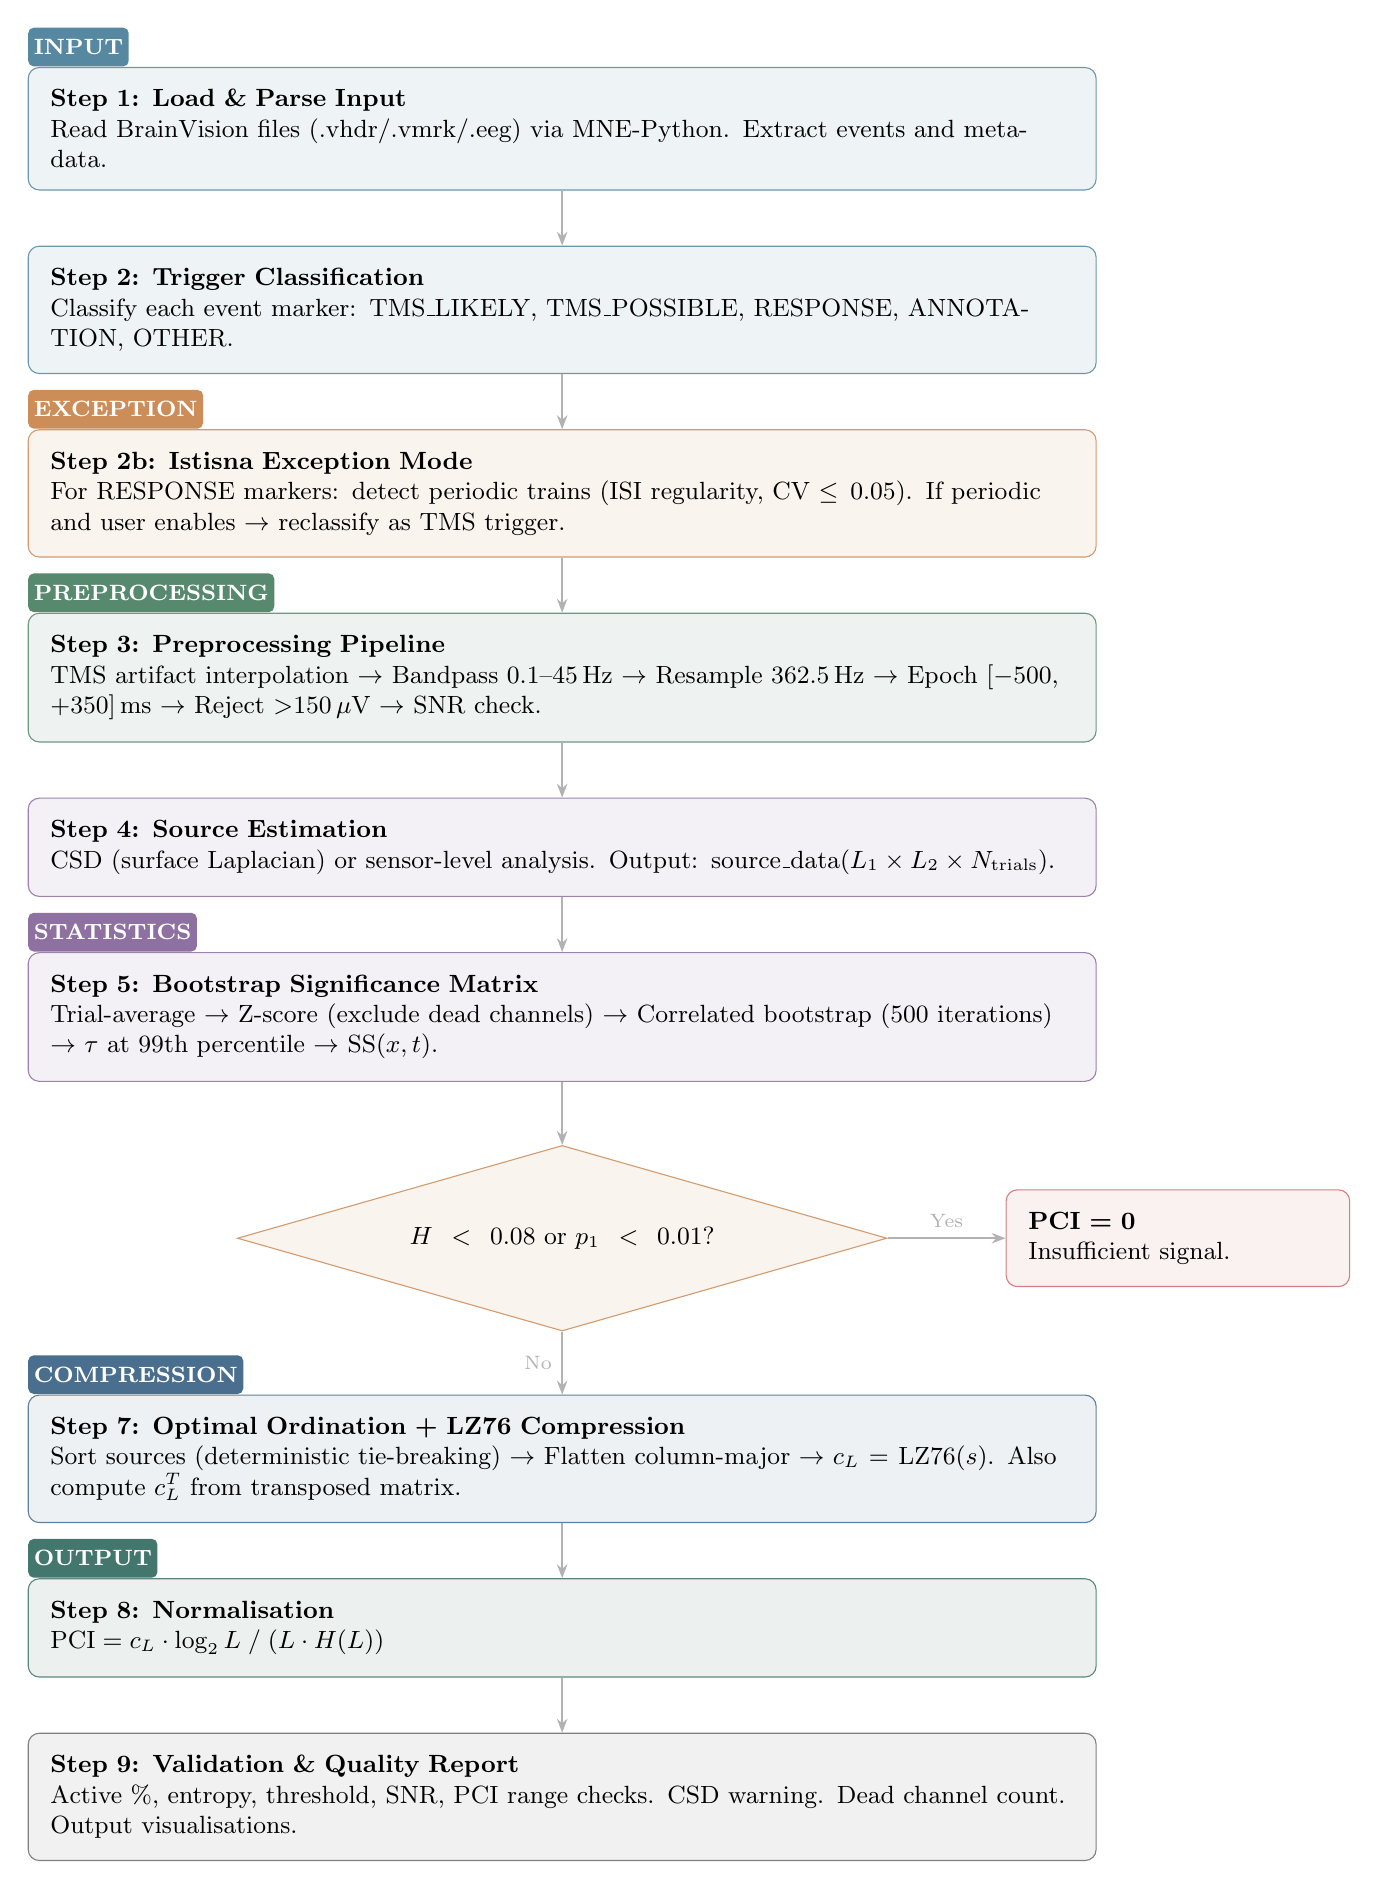
\begin{tikzpicture}[
  node distance=0.7cm,
  every node/.style={font=\small},
  block/.style={rectangle, rounded corners=4pt, draw=#1!70, fill=#1!8,
                text width=13cm, minimum height=1.1cm, align=left, inner sep=8pt,
                font=\small},
  decision/.style={diamond, draw=cOrange!70, fill=cOrange!8, aspect=3.5,
                   text width=6cm, align=center, inner sep=4pt, font=\small},
  arrow/.style={-{Stealth[length=5pt]}, thick, color=gray!60},
  label/.style={font=\scriptsize\bfseries, color=white, fill=#1!80, rounded corners=2pt,
                inner sep=2pt, minimum height=14pt},
]

% Nodes
\node[block=cBlue] (load)
  {\textbf{Step 1: Load \& Parse Input}\\
   Read BrainVision files (.vhdr/.vmrk/.eeg) via MNE-Python. Extract events and metadata.};

\node[block=cBlue, below=of load] (classify)
  {\textbf{Step 2: Trigger Classification}\\
   Classify each event marker: TMS\_LIKELY, TMS\_POSSIBLE, RESPONSE, ANNOTATION, OTHER.};

\node[block=cOrange, below=of classify] (istisna)
  {\textbf{Step 2b: Istisna Exception Mode}\\
   For RESPONSE markers: detect periodic trains (ISI regularity, CV $\leq 0.05$).
   If periodic and user enables $\rightarrow$ reclassify as TMS trigger.};

\node[block=cGreen, below=of istisna] (preproc)
  {\textbf{Step 3: Preprocessing Pipeline}\\
   TMS artifact interpolation $\rightarrow$ Bandpass 0.1--45\,Hz $\rightarrow$
   Resample 362.5\,Hz $\rightarrow$ Epoch [$-$500, +350]\,ms $\rightarrow$
   Reject $>$150\,$\mu$V $\rightarrow$ SNR check.};

\node[block=cPurple, below=of preproc] (source)
  {\textbf{Step 4: Source Estimation}\\
   CSD (surface Laplacian) or sensor-level analysis.
   Output: source\_data$(L_1 \times L_2 \times N_{\mathrm{trials}})$.};

\node[block=cPurple, below=of source] (boot)
  {\textbf{Step 5: Bootstrap Significance Matrix}\\
   Trial-average $\rightarrow$ Z-score (exclude dead channels) $\rightarrow$
   Correlated bootstrap (500 iterations) $\rightarrow$ $\tau$ at 99th percentile $\rightarrow$ SS$(x,t)$.};

\node[decision, below=0.8cm of boot] (gate)
  {$H < 0.08$ or $p_1 < 0.01$?};

\node[block=cRed, right=1.5cm of gate, text width=3.8cm, minimum height=0.8cm] (stop)
  {\textbf{PCI = 0}\\Insufficient signal.};

\node[block=cNavy, below=0.8cm of gate] (lz)
  {\textbf{Step 7: Optimal Ordination + LZ76 Compression}\\
   Sort sources (deterministic tie-breaking) $\rightarrow$ Flatten column-major $\rightarrow$
   $c_L = \mathrm{LZ76}(s)$. Also compute $c_L^T$ from transposed matrix.};

\node[block=cDarkGreen, below=of lz] (norm)
  {\textbf{Step 8: Normalisation}\\
   $\mathrm{PCI} = c_L \cdot \log_2 L \;/\; (L \cdot H(L))$};

\node[block=cGray, below=of norm] (valid)
  {\textbf{Step 9: Validation \& Quality Report}\\
   Active \%, entropy, threshold, SNR, PCI range checks.
   CSD warning. Dead channel count. Output visualisations.};

% Labels
\node[label=cBlue, anchor=south west] at (load.north west) {\footnotesize INPUT};
\node[label=cOrange, anchor=south west] at (istisna.north west) {\footnotesize EXCEPTION};
\node[label=cGreen, anchor=south west] at (preproc.north west) {\footnotesize PREPROCESSING};
\node[label=cPurple, anchor=south west] at (boot.north west) {\footnotesize STATISTICS};
\node[label=cNavy, anchor=south west] at (lz.north west) {\footnotesize COMPRESSION};
\node[label=cDarkGreen, anchor=south west] at (norm.north west) {\footnotesize OUTPUT};

% Arrows
\draw[arrow] (load) -- (classify);
\draw[arrow] (classify) -- (istisna);
\draw[arrow] (istisna) -- (preproc);
\draw[arrow] (preproc) -- (source);
\draw[arrow] (source) -- (boot);
\draw[arrow] (boot) -- (gate);
\draw[arrow] (gate) -- node[above, font=\scriptsize] {Yes} (stop);
\draw[arrow] (gate) -- node[left, font=\scriptsize] {No} (lz);
\draw[arrow] (lz) -- (norm);
\draw[arrow] (norm) -- (valid);

\end{tikzpicture}
}
\caption{Complete PCI algorithm flowchart showing the processing pipeline from raw EEG data
to the final PCI value with quality assessment.}
\label{fig:flowchart}
\end{figure}

% ══════════════════════════════════════════════════════════════════════
\section{Corrections and Improvements}
\label{sec:fixes}

The following issues were identified during a thorough code review against Casali et al.\ (2013)
and resolved:

\subsection{Critical Fixes}

\begin{enumerate}[leftmargin=2em]
  \item \textbf{Bootstrap resampling (correlated)}: The bootstrap previously drew independent
        random time indices per source, breaking spatial correlations. Fixed to draw a single
        set of indices shared across all sources, matching GMS \cite{nichols2002}.

  \item \textbf{Dead channel exclusion}: Sources with $\sigma \approx 0$ were previously
        floored to the 5th percentile of non-zero sigmas, inflating their z-scores. Now these
        channels are excluded entirely and assigned all-zero rows in $\mathbf{SS}$.

  \item \textbf{Permutation-invariant source sorting}: Added deterministic tie-breaking using
        row content as a binary number (Eq.~\ref{eq:rowvalue}), ensuring identical results
        regardless of the original row order.
\end{enumerate}

\subsection{Moderate Fixes}

\begin{enumerate}[leftmargin=2em]
  \item \textbf{Window overlap validation}: New warning when the TMS artifact interpolation
        window extends beyond the post-stimulus analysis start.

  \item \textbf{Threshold harmonisation}: \texttt{compute\_pci\_temporal} now uses the same
        quality gates (min\_entropy$\,= 0.08$, min\_p1$\,= 0.01$) as \texttt{compute\_pci}.

  \item \textbf{CSD documentation}: Prominent warnings added that CSD is not equivalent to
        full inverse-solution source reconstruction and that published thresholds may not apply.

  \item \textbf{Istisna CV threshold}: Raised from $0.02$ to $0.05$ to accommodate jitter
        from manual TMS triggering and low sampling rates.

  \item \textbf{Configurable random seed}: The bootstrap accepts a \texttt{seed} parameter
        (default 42, \texttt{None} for non-deterministic).
\end{enumerate}

% ══════════════════════════════════════════════════════════════════════
\section{Software Architecture}
\label{sec:arch}

\begin{table}[H]
\centering
\caption{Project file structure and responsibilities.}
\label{tab:files}
\begin{tabular}{@{}lll@{}}
\toprule
\textbf{File} & \textbf{Lines} & \textbf{Responsibility} \\
\midrule
\texttt{pci.py}       & ${\sim}950$  & Core algorithm: entropy, LZ76, bootstrap, PCI, trigger classification \\
\texttt{app.py}       & ${\sim}1230$ & Streamlit UI: file upload, parameter controls, visualisations \\
\texttt{test\_pci.py} & ${\sim}370$  & 41 unit tests covering all algorithm components \\
\bottomrule
\end{tabular}
\end{table}

\noindent
\textbf{Dependencies}: Python 3.8+, NumPy, MNE-Python, Streamlit, Matplotlib, pytest.

% ══════════════════════════════════════════════════════════════════════
\section{Test Suite}
\label{sec:tests}

The test suite (\texttt{tests/test\_pci.py}) contains 41 tests organised into 9 classes:

\begin{table}[H]
\centering
\caption{Test suite coverage summary.}
\label{tab:tests}
\begin{tabular}{@{}llc@{}}
\toprule
\textbf{Test Class} & \textbf{Tests} & \textbf{Count} \\
\midrule
\texttt{TestLZComplexity}          & LZ76 correctness on known sequences              & 7 \\
\texttt{TestEntropy}               & Binary entropy edge cases and known values        & 5 \\
\texttt{TestPCICore}               & PCI formula, zero matrices, simple patterns       & 5 \\
\texttt{TestTriggerClassification} & Keyword matching, count ranges, edge cases        & 7 \\
\texttt{TestResponseTrainDetection}& Periodicity detection, block splitting            & 5 \\
\texttt{TestValidation}            & Quality checks, trigger diagnostics               & 3 \\
\texttt{TestBootstrapSignificance} & Shape, correlated resampling, dead channels, seed & 5 \\
\texttt{TestWindowOverlap}         & Overlap warning, no-overlap silence               & 2 \\
\texttt{TestPCITemporal}           & Low entropy returns zeros, convergence            & 2 \\
\midrule
\textbf{Total}                     &                                                   & \textbf{41} \\
\bottomrule
\end{tabular}
\end{table}

All 41 tests pass as of the final verification (February 2026).

% ══════════════════════════════════════════════════════════════════════
\section{Future Work}
\label{sec:future}

\begin{itemize}[leftmargin=2em]
  \item \textbf{PCI$_{ST}$} (Comolatti et al., 2019 \cite{comolatti2019}): Implement the
        state-transition variant using SVD dimensionality reduction and recurrence
        quantification, which computes faster and has been validated on larger cohorts.
  \item \textbf{Bootstrap confidence intervals}: Report PCI uncertainty ranges via
        jackknife or bootstrap-of-bootstrap procedures.
  \item \textbf{ISI histogram}: Visual verification tool for istisna mode.
  \item \textbf{Additional file formats}: Support for EDF/BDF/EEGLAB beyond BrainVision.
  \item \textbf{Full inverse solution}: Integrate MNE's minimum-norm estimation for closer
        alignment with the original Casali et al.\ methodology.
\end{itemize}

% ══════════════════════════════════════════════════════════════════════
\begin{thebibliography}{9}

\bibitem{casali2013}
Casali AG, Gosseries O, Rosanova M, et al.
A theoretically based index of consciousness independent of sensory processing and behavior.
\emph{Science Translational Medicine}, 5(198):198ra105, 2013.

\bibitem{comolatti2019}
Comolatti R, Pigorini A, Casarotto S, et al.
A fast and general method to empirically estimate the complexity of brain responses to
transcranial and intracranial stimulations.
\emph{Brain Stimulation}, 12(5):1280--1289, 2019.

\bibitem{casarotto2016}
Casarotto S, Comanducci A, Rosanova M, et al.
Stratification of unresponsive patients by an independently validated index of brain complexity.
\emph{Annals of Neurology}, 80(5):718--729, 2016.

\bibitem{nichols2002}
Nichols TE, Holmes AP.
Nonparametric permutation tests for functional neuroimaging: A primer with examples.
\emph{Human Brain Mapping}, 15(1):1--25, 2002.

\bibitem{lempel1976}
Lempel A, Ziv J.
On the complexity of finite sequences.
\emph{IEEE Transactions on Information Theory}, 22(1):75--81, 1976.

\bibitem{kaspar1987}
Kaspar F, Schuster HG.
Easily calculable measure for the complexity of spatiotemporal patterns.
\emph{Physical Review A}, 36(2):842--848, 1987.

\bibitem{rogasch2017}
Rogasch NC, Sullivan C, Thomson RH, et al.
Analysing concurrent transcranial magnetic stimulation and electroencephalographic data:
A review and introduction to the open-source TESA software.
\emph{NeuroImage}, 147:934--951, 2017.

\end{thebibliography}

\end{document}
